\documentclass{lab_sheet}
\usepackage{booktabs,caption}
\usepackage[flushleft]{threeparttable}
\usepackage[defernumbers=true,sorting=none]{biblatex}
\DeclareBibliographyCategory{cited}
\AtEveryCitekey{\addtocategory{cited}{\thefield{entrykey}}}
\addbibresource{citation.bib}
\nocite{*} 
\renewcommand*{\thesubfigure}{\thefigure.\arabic{subfigure}}
\newcommand{\digitalpattern}[1]{
    \begin{tabular}{C{2cm}C{1cm}C{1cm}C{1cm}C{1cm}C{1cm}C{1cm}C{1cm}C{1cm}C{2cm}}
        \toprule
          Character & DP & g & f & e & d & c & b & a & HEX value\\
          \midrule
          #1
          \bottomrule
       \end{tabular}
}
\renewcommand{\lstlistlistingname}{Source Codes}
\renewcommand{\lstlistingname}{Code}
\begin{document}
    \titlePage{Interfacing 7-Segment LED Display with 8051/8052 Micro-controller}{October 9, 2020}
    \pagenumbering{gobble}
    \tableofcontents
    \pagebreak
    \listoffigures
    \pagebreak
    \listoftables
    \pagebreak
    \lstlistoflistings
    \pagebreak
    \pagenumbering{arabic}
    \section{Introduction}
    \subsection{MCS-51 Family Microcontroller Chips}
    Based on the Harvard architecture of designing ICs, the MCS-51 microcontroller chips were originally developed by Intel to be used in small embedded systems. The MCS-51 chips now use Complementary Metal-Oxide Semiconductor (CMOS) instead of the original NMOS, and are thus known as 80C51 chips. Texas Instruments, Atmel, Dallas Semiconductors, Silicon Laboratories, ASTX, and many more distributors manufacture and sell the MCS-51 family microcontroller chips.\\
    The different features of the 8051 microcontroller are: 
    \begin{itemize}
        \item 8-bit ALU, Accumulator and Registers, making it an 8-bit microcontroller.
        \item 4KB of ROM for the programs, also called program memory.
        \item 8-bit data bus meaning that it can access 8 bits of data in one operation.
        \item 128 Bytes of RAM for the variables, also called data memory.
        \item 32 I/O lines, i.e. 4 ports with 8 lines each.
        \item 16-bit address bus meaning that it can access 65536 locations of RAM and ROM.
        \item 2 16-bit timers/counters.
        \item 1 full-duplex serial port for serial communication (UART).
        \item 6 interrupt sources(2 external interrupts, 2 timer interrupts \& 2 serial interrupts).
        \end{itemize}
    \subsection{7-Segment LED Display}
    7-segment LED display is a basic electronic device that is made up of 7 led segments each arranged in such a way that specific configurations of these LEDs allow certain alpha-numeric characters to be displayed on the device. Most 7-segment LEDs also contain an additional LED to indicate the decimal point when two or more 7-segment LED displays are used in conjuction. Each of the seven LEDs have a positional reference with pin outs generally being named as a, b, c, d, e, f, g and DP. One end of all the LEDs are commoned out whereas other end is provided with a proper biasing voltage to either turn on or off the segment depending on the terminal polarity. Forward biasing of the appropriate LED segments are used to display the desired character or pattern. Widely used in digital clocks, small-scale calculators, electronic meters and digital display units, the 7-segment LED displays serve a handy purpose in digital electronics.\\
    Sice multiplexing 7-segment displays allows for less number of port connections, less power consumptions and more interfaces, multiplexed 7-segment LED displays are widely used. \cite{rathod2020a} addresses the multiplexed 7-segment display interfacing with a 8051 microcontroller.
    \subsubsection{Types of 7-Segment LED Display}
    \subsubsection*{Common-Cathode}
    7-segment LED display where the cathode terminal of the LEDs is made common is called a common cathode (CC) 7-segment LED display. The common cathode terminal is connected to a LOW logic where as individual anode terminals are connected to the HIGH logic through a current limiting resistor as necessary. Certain illumination combinations of the LED segments display the desired character.
    \begin{figure}[H]
        \centering
        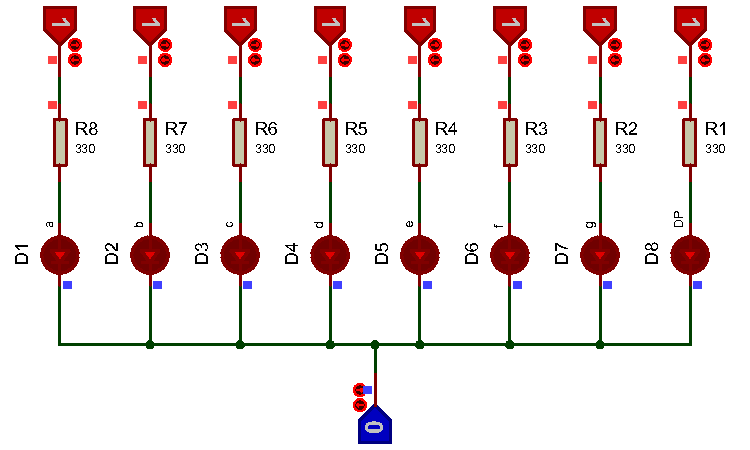
\includegraphics[scale=1]{../Figures/led1}
        \caption{Common-Cathode (CC) configuration for a 7-segment display}
        \label{fig:cc}
        \end{figure}
        \subsubsection*{Common-Anode}
        7-segment LED display where the anode terminal of the LEDs is made common is called a common anode (CA) 7-segment LED display. The common anode terminal is connected to a HIGH logic where as individual cathode terminals are connected to the LOW logic through a current limiting resistor as necessary. Certain illumination combinations of the LED segments display the desired character.
        \begin{figure}[H]
            \centering
            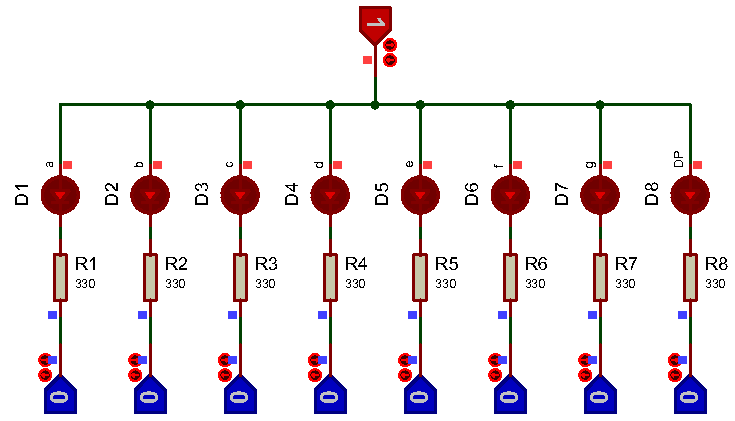
\includegraphics[scale=1]{../Figures/led2}
            \caption{Common-Anode (CA) configuration for a 7-segment display}
            \label{fig:ca}
            \end{figure}
    \subsubsection{Digital Drive Pattern}
    For a common cathode 7-segment LED display, the segments a through g and DP must be provided HIGH logic in order to be turned on. Likewise, for a common anode 7-segment LED display, the segments a through g and DP must be provided LOW logic in order to be turned on. The different combinations that are to be used to display certain characters are called digital drive pattern. The table that stores these patterns is called a lookup table.
    \begin{table}[H]
        \centering
        \begin{threeparttable}
        \digitalpattern{0 & 0 & 0 & 1 & 1 & 1 & 1 & 1 & 1 & 3F H\\
        1 & 0 & 0 & 0 & 0 & 0 & 1 & 1 & 0 & 06 H\\
        2 & 0 & 1 & 0 & 1 & 1 & 0 & 1 & 1 & 5B H\\
        3 & 0 & 1 & 0 & 0 & 1 & 1 & 1 & 1 & 4F H\\
        4 & 0 & 1 & 1 & 0 & 0 & 1 & 1 & 0 & 66 H\\
        5 & 0 & 1 & 1 & 0 & 1 & 1 & 0 & 1 & 6D H\\
        6 & 0 & 1 & 1 & 1 & 1 & 1 & 0 & 1 & 7D H\\
        7 & 0 & 0 & 0 & 0 & 0 & 1 & 1 & 1 & 07 H\\
        8 & 0 & 1 & 1 & 1 & 1 & 1 & 1 & 1 & 7F H\\
        9 & 0 & 1 & 1 & 0 & 1 & 1 & 1 & 1 & 6F H\\
        E & 0 & 1 & 1 & 1 & 1 & 0 & 0 & 1 & 79 H\\}
  \begin{tablenotes}
    \small
    \item Note: For displaying any character along with a decimal point, the HEX value should be ORed with 80 H.
  \end{tablenotes}
  \caption{Lookup table for a Common-Cathode 7-segment display}
  \label{tbl:cc}
        \end{threeparttable}
    \end{table}
    \begin{table}[H]
        \centering
        \begin{threeparttable}
        \digitalpattern{
        0 & 1 & 1 & 0 & 0 & 0 & 0 & 0 & 0 & C0 H \\
        1 & 1 & 1 & 1 & 1 & 1 & 0 & 0 & 1 & F9 H \\
        2 & 1 & 0 & 1 & 0 & 0 & 1 & 0 & 0 & A4 H \\
        3 & 1 & 0 & 1 & 1 & 0 & 0 & 0 & 0 & B0 H \\
        4 & 1 & 0 & 0 & 1 & 1 & 0 & 0 & 1 & 99 H \\
        5 & 1 & 0 & 0 & 1 & 0 & 0 & 1 & 0 & 92 H \\
        6 & 1 & 0 & 0 & 0 & 0 & 0 & 1 & 0 & 82 H \\
        7 & 1 & 1 & 1 & 1 & 1 & 0 & 0 & 0 & F8 H \\
        8 & 1 & 0 & 0 & 0 & 0 & 0 & 0 & 0 & 80 H \\
        9 & 1 & 0 & 0 & 1 & 0 & 0 & 0 & 0 & 90 H \\
        E & 1 & 0 & 0 & 0 & 0 & 1 & 1 & 0 & 86 H\\}
        \begin{tablenotes}
            \small
            \item Note: For displaying any character along with a decimal point, the HEX value should be ANDed with 7F H.
          \end{tablenotes}
  \caption{Lookup table for a Common-Anode 7-segment display}
  \label{tbl:ca}
\end{threeparttable}
    \end{table}
    \section{Objectives}
    The primary objective of this lab experiment is to understand the various steps involved while interfacing a 7-segment LED display with the 8051/8052 microcontroller. The interfacing knowledge will enable us to write assembly and Embedded C code for the 8051/8052 microcontroller capable of:
    \begin{itemize}
        \item Displaying non-multiplexed and multiplexed output on the 7-segment LED units.
        \item Displaying static and scrolling outputs on the 7-segment LED units.
    \end{itemize}
    \section{Lab Experiment Enviornment}
    The lab experiments will be performed virtually via various simulation softwares. The basic usages of these tools will allow us to visualize and tally the interfacing of a 7-segment LED display with the 8051/8052 microcontroller. Due to a simulated environment, the observations are carefully selected to represent the problems with maximum efficiency.
    \subsection{Circuit Simulation}
    A profession PCB layout, circuit design and simulation tool, Proteus Design Suite was used to simulate the interface between a 8052 microcontroller and a common cathode 7-segment LED display. Additional electronic components such as resistors, resistor bus, transistors were also used to attain the circuit shown in Figure~\ref{fig:proteus}.
    \subsection{Code Editor and Compiler}
    KEIL $\mu$Vision, which is a product of the ARM Ltd. was used as the code editor for the assembly and embeddded C codes for the different lab problems. KEIL products include C/C++ compilers, debuggers, integrated development and simulation environments, RTOS and
    middleware libraries, and evaluation boards for ARM, Cortex-M, Cortex-R4, 8051, C166, and 251 processor families. The compiler built-in with KEIL converts the codes into respective HEX codes that are understandable by the microcontroller.
    \begin{figure}[H]
        \centering
        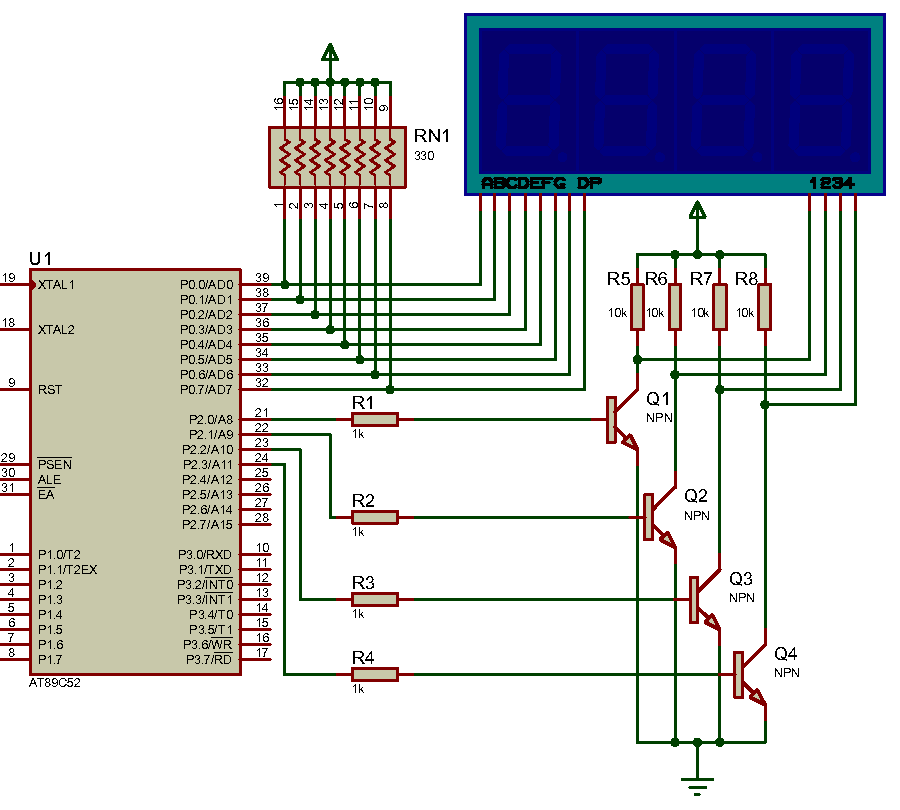
\includegraphics[scale=0.9]{../Figures/proteus}
        \caption{Circuit diagram for Proteus simulation}
        \label{fig:proteus}
    \end{figure}
    \section{Lab Problems}
    \problem{Write a code to design a single digit decimal counter that counts up from 0 to 9 and back to 0. This process should repeat indefinitely.}
    \code{lab_2_a}
    \problem{Write a code to design a double digit decimal counter that counts up from 00 to 20 and back to 00 indefinitely.}
    \code{lab_2_b}
    \problem{Write a code to display the first (N) numbers of the Fibonacci sequence, where the number (N) must be stored in a memory location and can be any integer from 1 to 10. The sequence should repeat indefinitely.}
    \code{lab_2_c}
    \problem{Write a code to generate the multiplication table of a number (N) stored in a memory location which can be any integer from 1 to 10. Repeat the sequence indefinitely.}
    \code{lab_2_d}
    \problem{Write a code to display your roll numbers in static format. Each student roll number should be of four characters. Display of student roll number should repeat indefinitely.}
    \code{lab_2_e}
    \problem{Write a code to display your roll number in scrolling format, separated by using decimal point. Roll number should be scrolled towards the left and repeated indefinitely.}
    \code{lab_2_f}
    \section{Observations}
    The observations for the 7-segment LED display are taken from Proteus VSM debugging. The different characters for a multiplexed display are actually displayed in quick succession with very less delay in order to trigger the persistence of vision of human eye, enabling us to use a single bus of segments to control multiplexed LED segments. The observations are taken based on a common cathode 7-segment LED display, but similar results can be obtained for a common anode type by using the look up table shown in Table~\ref{tbl:ca}.
    \subsection*{Problem 1}
\begin{figure}[H]
\begin{subfigure}{.33\textwidth}
  \centering
  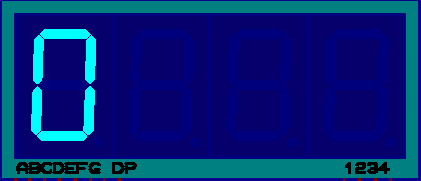
\includegraphics[frame,width=.9\linewidth]{../Figures/s0}  
  \label{fig:prob1-a}
  \caption{}
\end{subfigure}
\begin{subfigure}{.33\textwidth}
  \centering
  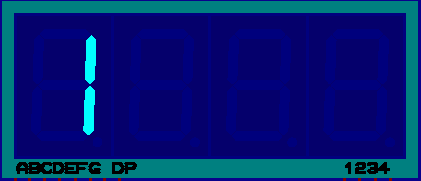
\includegraphics[frame,width=.9\linewidth]{../Figures/s1}  
  \label{fig:prob1-b}
  \caption{}
\end{subfigure}
\begin{subfigure}{.33\textwidth}
  \centering
    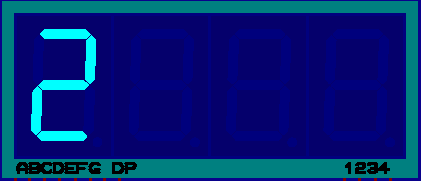
\includegraphics[frame,width=.9\linewidth]{../Figures/s2}  
  \label{fig:prob1-c}
  \caption{}
\end{subfigure}
\newline
\begin{subfigure}{.33\textwidth}
  \centering
  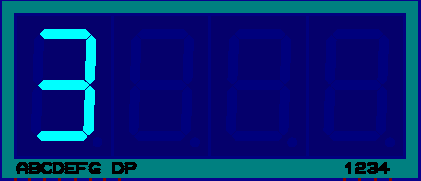
\includegraphics[frame,width=.9\linewidth]{../Figures/s3}     
  \caption{}
  \label{fig:prob1-d}
\end{subfigure}
\begin{subfigure}{.33\textwidth}
  \centering
  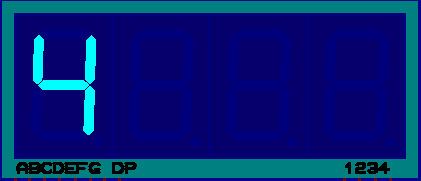
\includegraphics[frame,width=.9\linewidth]{../Figures/s4}   
  \caption{}
  \label{fig:prob1-e}
\end{subfigure}
\begin{subfigure}{.33\textwidth}
  \centering
  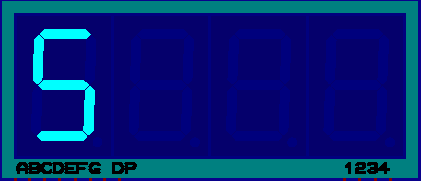
\includegraphics[frame,width=.9\linewidth]{../Figures/s5}   
  \caption{}
  \label{fig:prob1-f}
\end{subfigure}
\newline
\begin{subfigure}{.33\textwidth}
    \centering
    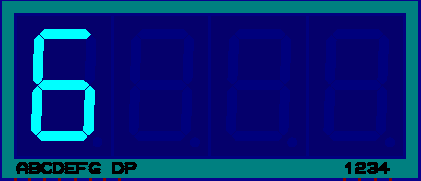
\includegraphics[frame,width=.9\linewidth]{../Figures/s6}   
    \caption{}
    \label{fig:prob1-g}
  \end{subfigure}
  \begin{subfigure}{.33\textwidth}
    \centering
    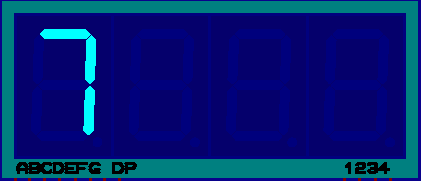
\includegraphics[frame,width=.9\linewidth]{../Figures/s7}   
    \caption{}
    \label{fig:prob1-h}
  \end{subfigure}
  \begin{subfigure}{.33\textwidth}
    \centering
    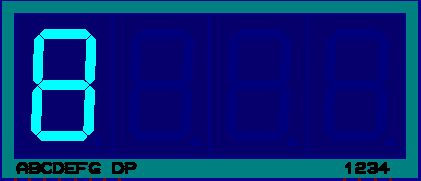
\includegraphics[frame,width=.9\linewidth]{../Figures/s8}   
    \caption{}
    \label{fig:prob1-i}
  \end{subfigure}
  \newline
  \begin{subfigure}{.33\textwidth}
    \centering
    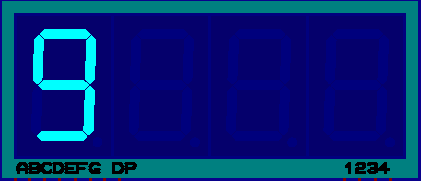
\includegraphics[frame,width=.9\linewidth]{../Figures/s9}   
    \caption{}
    \label{fig:prob1-j}
  \end{subfigure}
  \begin{subfigure}{.33\textwidth}
    \centering
    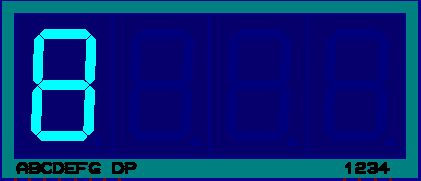
\includegraphics[frame,width=.9\linewidth]{../Figures/s8}   
    \caption{}
    \label{fig:prob1-k}
  \end{subfigure}
  \begin{subfigure}{.33\textwidth}
    \centering
    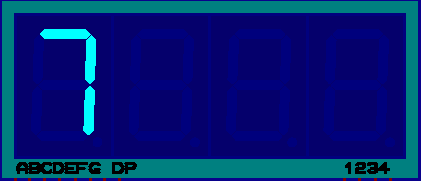
\includegraphics[frame,width=.9\linewidth]{../Figures/s7}   
    \caption{}
    \label{fig:prob1-l}
  \end{subfigure}
\caption{Observation for Problem 1}
\label{fig:prob1}
\end{figure}
\begin{figure}[H]\ContinuedFloat
      \begin{subfigure}{.33\textwidth}
        \centering
        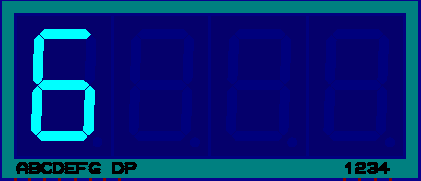
\includegraphics[frame,width=.9\linewidth]{../Figures/s6}   
        \caption{}
        \label{fig:prob1-m}
      \end{subfigure}
      \begin{subfigure}{.33\textwidth}
        \centering
        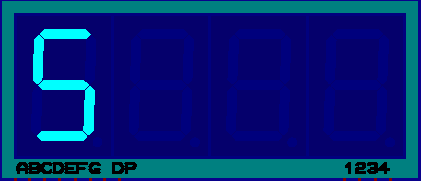
\includegraphics[frame,width=.9\linewidth]{../Figures/s5}   
        \caption{}
        \label{fig:prob1-n}
      \end{subfigure}
      \begin{subfigure}{.33\textwidth}
        \centering
        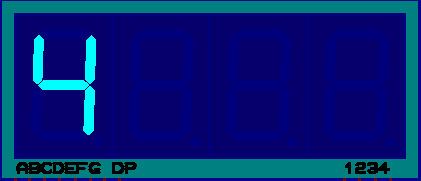
\includegraphics[frame,width=.9\linewidth]{../Figures/s4}   
        \caption{}
        \label{fig:prob1-o}
      \end{subfigure}
      \newline
      \begin{subfigure}{.33\textwidth}
        \centering
        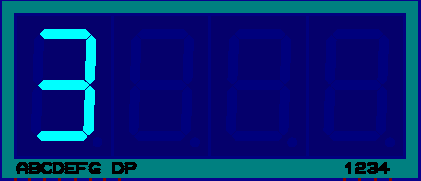
\includegraphics[frame,width=.9\linewidth]{../Figures/s3}   
        \caption{}
        \label{fig:prob1-p}
      \end{subfigure}
      \begin{subfigure}{.33\textwidth}
        \centering
        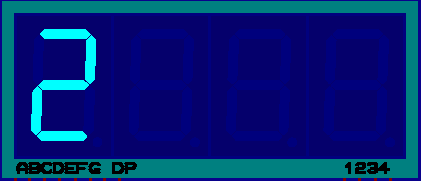
\includegraphics[frame,width=.9\linewidth]{../Figures/s2}   
        \caption{}
        \label{fig:prob1-q}
      \end{subfigure}
      \begin{subfigure}{.33\textwidth}
        \centering
        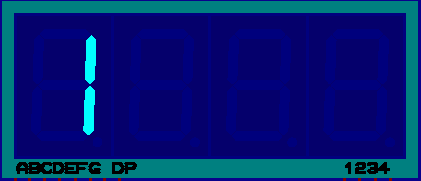
\includegraphics[frame,width=.9\linewidth]{../Figures/s1}   
        \caption{}
        \label{fig:prob1-r}
      \end{subfigure}
      \newline
      \hspace*{\fill}
      \begin{subfigure}{.33\textwidth}
        \centering
        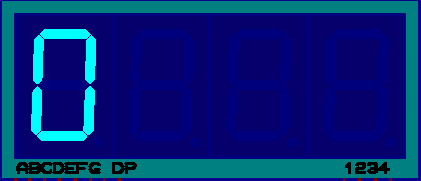
\includegraphics[frame,width=.9\linewidth]{../Figures/s0}   
        \caption{}
        \label{fig:prob1-s}
      \end{subfigure}
      \hspace*{\fill}
      \caption*{Figure~\ref{fig:prob1}:~Observation for Problem 1 (continued)}
\end{figure}
Figure~\ref{fig:prob1} shows the observations for Problem 1. The digits 0 to 9 are displayed on the first 7-segment LED display and then the display returns 8 to 0. That is to say, single digit decimal counter that counts up from 0 to 9 and back to 0 is observed. The loop continues indefinitely but only one cycle is presented in this report.
\subsection*{Problem 2}
\begin{figure}[H]
    \begin{subfigure}{.33\textwidth}
      \centering
      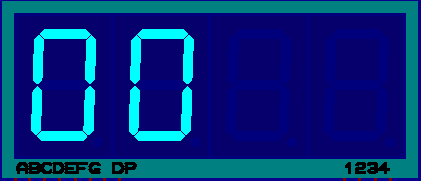
\includegraphics[frame,width=.9\linewidth]{../Figures/d0}  
      \label{fig:prob2-a}
      \caption{}
    \end{subfigure}
    \begin{subfigure}{.33\textwidth}
      \centering
      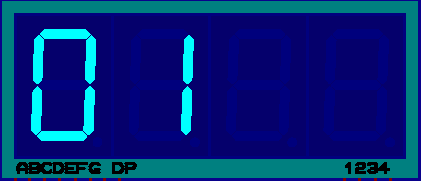
\includegraphics[frame,width=.9\linewidth]{../Figures/d1}  
      \label{fig:prob2-b}
      \caption{}
    \end{subfigure}
    \begin{subfigure}{.33\textwidth}
      \centering
        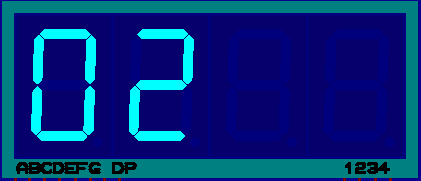
\includegraphics[frame,width=.9\linewidth]{../Figures/d2}  
      \label{fig:prob2-c}
      \caption{}
    \end{subfigure}
    \newline
    \begin{subfigure}{.33\textwidth}
      \centering
      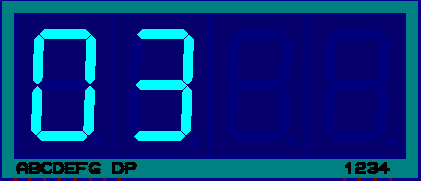
\includegraphics[frame,width=.9\linewidth]{../Figures/d3}     
      \caption{}
      \label{fig:prob2-d}
    \end{subfigure}
    \begin{subfigure}{.33\textwidth}
      \centering
      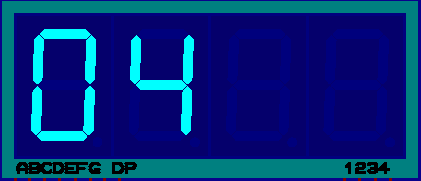
\includegraphics[frame,width=.9\linewidth]{../Figures/d4}   
      \caption{}
      \label{fig:prob2-e}
    \end{subfigure}
    \begin{subfigure}{.33\textwidth}
      \centering
      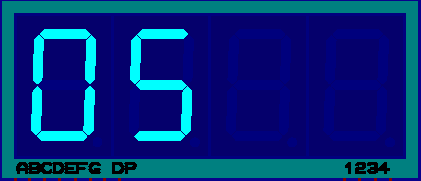
\includegraphics[frame,width=.9\linewidth]{../Figures/d5}   
      \caption{}
      \label{fig:prob2-f}
    \end{subfigure}
    \newline
    \begin{subfigure}{.33\textwidth}
        \centering
        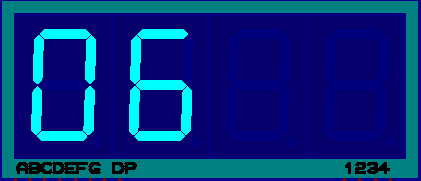
\includegraphics[frame,width=.9\linewidth]{../Figures/d6}   
        \caption{}
        \label{fig:prob2-g}
      \end{subfigure}
      \begin{subfigure}{.33\textwidth}
        \centering
        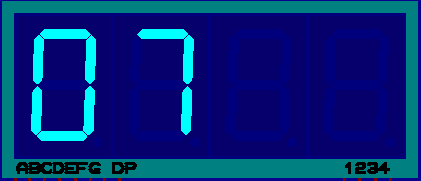
\includegraphics[frame,width=.9\linewidth]{../Figures/d7}   
        \caption{}
        \label{fig:prob2-h}
      \end{subfigure}
      \begin{subfigure}{.33\textwidth}
        \centering
        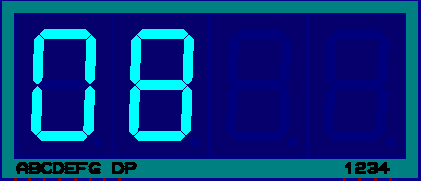
\includegraphics[frame,width=.9\linewidth]{../Figures/d8}   
        \caption{}
        \label{fig:prob2-i}
      \end{subfigure}
    \caption{Observation for Problem 2}
    \label{fig:prob2}
    \end{figure}
    \begin{figure}[H]\ContinuedFloat
        \begin{subfigure}{.33\textwidth}
          \centering
          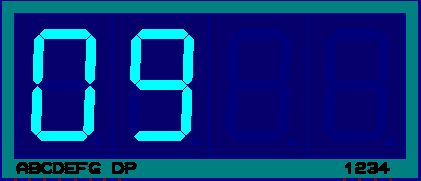
\includegraphics[frame,width=.9\linewidth]{../Figures/d9}   
          \caption{}
          \label{fig:prob2-j}
        \end{subfigure}
        \begin{subfigure}{.33\textwidth}
          \centering
          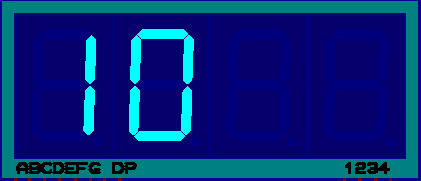
\includegraphics[frame,width=.9\linewidth]{../Figures/d10}   
          \caption{}
          \label{fig:prob2-k}
        \end{subfigure}
        \begin{subfigure}{.33\textwidth}
          \centering
          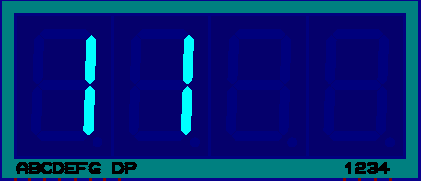
\includegraphics[frame,width=.9\linewidth]{../Figures/d11}   
          \caption{}
          \label{fig:prob2-l}
        \end{subfigure}
        \newline
        \begin{subfigure}{.33\textwidth}
          \centering
          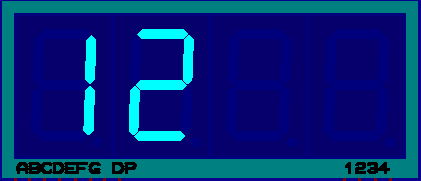
\includegraphics[frame,width=.9\linewidth]{../Figures/d12}   
          \caption{}
          \label{fig:prob2-m}
        \end{subfigure}
        \begin{subfigure}{.33\textwidth}
          \centering
          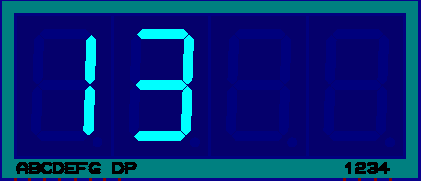
\includegraphics[frame,width=.9\linewidth]{../Figures/d13}   
          \caption{}
          \label{fig:prob2-n}
        \end{subfigure}
        \begin{subfigure}{.33\textwidth}
          \centering
          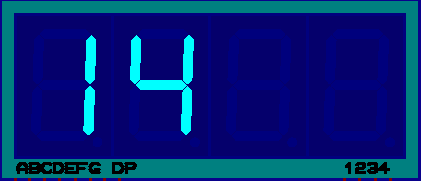
\includegraphics[frame,width=.9\linewidth]{../Figures/d14}   
          \caption{}
          \label{fig:prob2-o}
        \end{subfigure}
        \newline
        \begin{subfigure}{.33\textwidth}
          \centering
          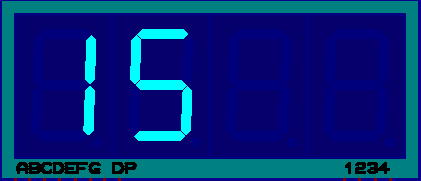
\includegraphics[frame,width=.9\linewidth]{../Figures/d15}   
          \caption{}
          \label{fig:prob2-p}
        \end{subfigure}
        \begin{subfigure}{.33\textwidth}
          \centering
          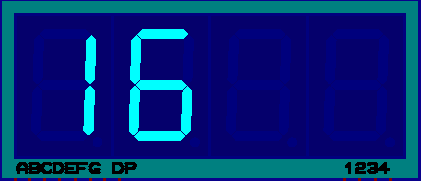
\includegraphics[frame,width=.9\linewidth]{../Figures/d16}   
          \caption{}
          \label{fig:prob2-q}
        \end{subfigure}
        \begin{subfigure}{.33\textwidth}
          \centering
          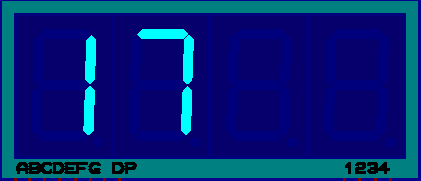
\includegraphics[frame,width=.9\linewidth]{../Figures/d17}   
          \caption{}
          \label{fig:prob2-r}
        \end{subfigure}
        \newline
        \begin{subfigure}{.33\textwidth}
          \centering
          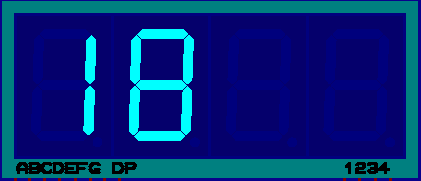
\includegraphics[frame,width=.9\linewidth]{../Figures/d18}   
          \caption{}
          \label{fig:prob2-s}
        \end{subfigure}
        \begin{subfigure}{.33\textwidth}
          \centering
          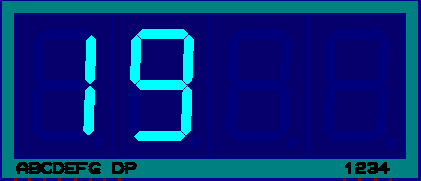
\includegraphics[frame,width=.9\linewidth]{../Figures/d19}   
          \caption{}
          \label{fig:prob2-t}
        \end{subfigure}
        \begin{subfigure}{.33\textwidth}
          \centering
          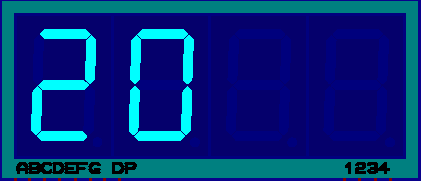
\includegraphics[frame,width=.9\linewidth]{../Figures/d20}   
          \caption{}
          \label{fig:prob2-u}
        \end{subfigure}
        \newline
        \begin{subfigure}{.33\textwidth}
            \centering
            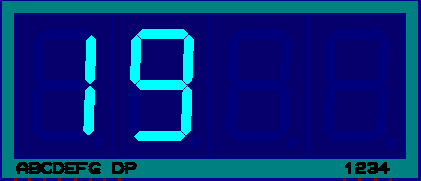
\includegraphics[frame,width=.9\linewidth]{../Figures/d19}   
            \caption{}
            \label{fig:prob2-v}
          \end{subfigure}
          \begin{subfigure}{.33\textwidth}
            \centering
            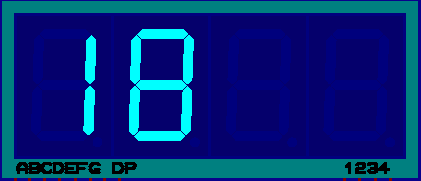
\includegraphics[frame,width=.9\linewidth]{../Figures/d18}   
            \caption{}
            \label{fig:prob2-w}
          \end{subfigure}
          \begin{subfigure}{.33\textwidth}
            \centering
            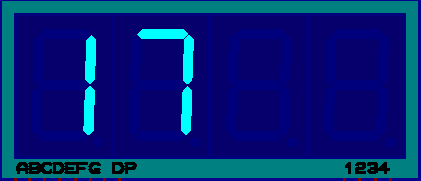
\includegraphics[frame,width=.9\linewidth]{../Figures/d17}   
            \caption{}
            \label{fig:prob2-x}
          \end{subfigure}
          \newline
          \begin{subfigure}{.33\textwidth}
            \centering
            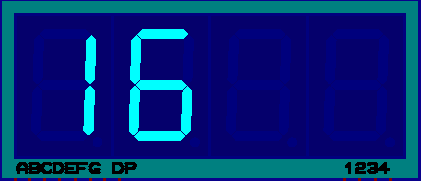
\includegraphics[frame,width=.9\linewidth]{../Figures/d16}   
            \caption{}
            \label{fig:prob2-y}
          \end{subfigure}
          \begin{subfigure}{.33\textwidth}
            \centering
            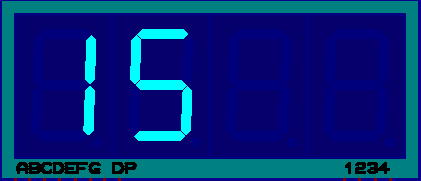
\includegraphics[frame,width=.9\linewidth]{../Figures/d15}   
            \caption{}
            \label{fig:prob2-z}
          \end{subfigure}
          \begin{subfigure}{.33\textwidth}
            \centering
            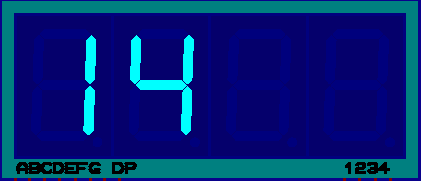
\includegraphics[frame,width=.9\linewidth]{../Figures/d14}   
            \caption{}
            \label{fig:prob2-a1}
          \end{subfigure}
          \newline
          \begin{subfigure}{.33\textwidth}
            \centering
            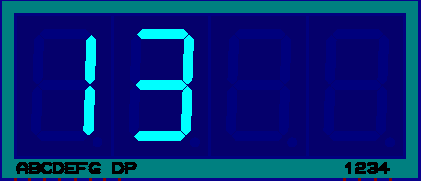
\includegraphics[frame,width=.9\linewidth]{../Figures/d13}   
            \caption{}
            \label{fig:prob2-a2}
          \end{subfigure}
          \begin{subfigure}{.33\textwidth}
            \centering
            \includegraphics[frame,width=.9\linewidth]{../Figures/d12}   
            \caption{}
            \label{fig:prob2-a3}
          \end{subfigure}
          \begin{subfigure}{.33\textwidth}
            \centering
            \includegraphics[frame,width=.9\linewidth]{../Figures/d11}   
            \caption{}
            \label{fig:prob2-a4}
          \end{subfigure}
          \newline
          \begin{subfigure}{.33\textwidth}
            \centering
            \includegraphics[frame,width=.9\linewidth]{../Figures/d10}   
            \caption{}
            \label{fig:prob2-a5}
          \end{subfigure}
          \begin{subfigure}{.33\textwidth}
            \centering
            \includegraphics[frame,width=.9\linewidth]{../Figures/d9}   
            \caption{}
            \label{fig:prob2-a6}
          \end{subfigure}
          \begin{subfigure}{.33\textwidth}
            \centering
            \includegraphics[frame,width=.9\linewidth]{../Figures/d8}   
            \caption{}
            \label{fig:prob2-a7}
          \end{subfigure}
          \caption*{Figure~\ref{fig:prob2}:~Observation for Problem 2 (continued)}
    \end{figure}
    \begin{figure}[H]\ContinuedFloat
        \begin{subfigure}{.33\textwidth}
            \centering
            \includegraphics[frame,width=.9\linewidth]{../Figures/d7}   
            \caption{}
            \label{fig:prob2-a8}
          \end{subfigure}
          \begin{subfigure}{.33\textwidth}
            \centering
            \includegraphics[frame,width=.9\linewidth]{../Figures/d6}   
            \caption{}
            \label{fig:prob2-a9}
          \end{subfigure}
          \begin{subfigure}{.33\textwidth}
            \centering
            \includegraphics[frame,width=.9\linewidth]{../Figures/d5}   
            \caption{}
            \label{fig:prob2-a10}
          \end{subfigure}
          \newline
          \begin{subfigure}{.33\textwidth}
            \centering
            \includegraphics[frame,width=.9\linewidth]{../Figures/d4}   
            \caption{}
            \label{fig:prob2-a11}
          \end{subfigure}
          \begin{subfigure}{.33\textwidth}
            \centering
            \includegraphics[frame,width=.9\linewidth]{../Figures/d3}   
            \caption{}
            \label{fig:prob2-a12}
          \end{subfigure}
          \begin{subfigure}{.33\textwidth}
            \centering
            \includegraphics[frame,width=.9\linewidth]{../Figures/d2}   
            \caption{}
            \label{fig:prob2-a13}
          \end{subfigure}
          \newline
          \hspace*{\fill}
          \begin{subfigure}{.33\textwidth}
            \centering
            \includegraphics[frame,width=.9\linewidth]{../Figures/d1}   
            \caption{}
            \label{fig:prob2-a14}
          \end{subfigure}
          \begin{subfigure}{.33\textwidth}
            \centering
            \includegraphics[frame,width=.9\linewidth]{../Figures/d0}   
            \caption{}
            \label{fig:prob2-a15}
          \end{subfigure}
          \hspace*{\fill}
        \caption*{Figure~\ref{fig:prob2}:~Observation for Problem 2 (continued)}
    \end{figure}
    Figure~\ref{fig:prob2} shows the observations for Problem 2. The digits 00 to 20 are displayed on the first and second 7-segment LED display and then the display returns 19 to 00. That is to say, double digit decimal counter that counts up from 00 to 20 and back to 00 is observed. The loop continues indefinitely but only one cycle is presented in this report.
    \subsection*{Problem 3}
    \begin{figure}[H]
        \begin{subfigure}{.33\textwidth}
          \centering
          \includegraphics[frame,width=.9\linewidth]{../Figures/f0}  
          \label{fig:prob3-a}
          \caption{}
        \end{subfigure}
        \begin{subfigure}{.33\textwidth}
          \centering
          \includegraphics[frame,width=.9\linewidth]{../Figures/f1}  
          \label{fig:prob3-b}
          \caption{}
        \end{subfigure}
        \begin{subfigure}{.33\textwidth}
          \centering
            \includegraphics[frame,width=.9\linewidth]{../Figures/f1}  
          \label{fig:prob3-c}
          \caption{}
        \end{subfigure}
        \newline
        \begin{subfigure}{.33\textwidth}
          \centering
          \includegraphics[frame,width=.9\linewidth]{../Figures/f2}     
          \caption{}
          \label{fig:prob3-d}
        \end{subfigure}
        \begin{subfigure}{.33\textwidth}
          \centering
          \includegraphics[frame,width=.9\linewidth]{../Figures/f3}   
          \caption{}
          \label{fig:prob3-e}
        \end{subfigure}
        \begin{subfigure}{.33\textwidth}
          \centering
          \includegraphics[frame,width=.9\linewidth]{../Figures/f5}   
          \caption{}
          \label{fig:prob3-f}
        \end{subfigure}
        \newline
        \begin{subfigure}{.33\textwidth}
            \centering
            \includegraphics[frame,width=.9\linewidth]{../Figures/f8}   
            \caption{}
            \label{fig:prob3-g}
          \end{subfigure}
          \begin{subfigure}{.33\textwidth}
            \centering
            \includegraphics[frame,width=.9\linewidth]{../Figures/f13}   
            \caption{}
            \label{fig:prob3-h}
          \end{subfigure}
          \begin{subfigure}{.33\textwidth}
            \centering
            \includegraphics[frame,width=.9\linewidth]{../Figures/f21}   
            \caption{}
            \label{fig:prob3-i}
          \end{subfigure}
        \caption{Observation for Problem 3}
        \label{fig:prob3}
        \end{figure}
        Figure~\ref{fig:prob3} shows the observations for Problem 3. The fibonacci series up to N=9 terms is shown on the display. The display continually re-runs but only one cycle is included in this report.
        \subsection*{Problem 4}
        \begin{figure}[H]
            \begin{subfigure}{.33\textwidth}
              \centering
              \includegraphics[frame,width=.9\linewidth]{../Figures/m8}  
              \label{fig:prob4-a}
              \caption{}
            \end{subfigure}
            \begin{subfigure}{.33\textwidth}
              \centering
              \includegraphics[frame,width=.9\linewidth]{../Figures/m16}  
              \label{fig:prob4-b}
              \caption{}
            \end{subfigure}
            \begin{subfigure}{.33\textwidth}
              \centering
                \includegraphics[frame,width=.9\linewidth]{../Figures/m24}  
              \label{fig:prob4-c}
              \caption{}
            \end{subfigure}
            \newline
            \begin{subfigure}{.33\textwidth}
              \centering
              \includegraphics[frame,width=.9\linewidth]{../Figures/m32}     
              \caption{}
              \label{fig:prob4-d}
            \end{subfigure}
            \begin{subfigure}{.33\textwidth}
              \centering
              \includegraphics[frame,width=.9\linewidth]{../Figures/m40}   
              \caption{}
              \label{fig:prob4-e}
            \end{subfigure}
            \begin{subfigure}{.33\textwidth}
              \centering
              \includegraphics[frame,width=.9\linewidth]{../Figures/m48}   
              \caption{}
              \label{fig:prob4-f}
            \end{subfigure}
            \newline
            \begin{subfigure}{.33\textwidth}
                \centering
                \includegraphics[frame,width=.9\linewidth]{../Figures/m56}   
                \caption{}
                \label{fig:prob4-g}
              \end{subfigure}
              \begin{subfigure}{.33\textwidth}
                \centering
                \includegraphics[frame,width=.9\linewidth]{../Figures/m64}   
                \caption{}
                \label{fig:prob4-h}
              \end{subfigure}
              \begin{subfigure}{.33\textwidth}
                \centering
                \includegraphics[frame,width=.9\linewidth]{../Figures/m72}   
                \caption{}
                \label{fig:prob4-i}
              \end{subfigure}
              \newline
              \hspace*{\fill}
              \begin{subfigure}{.33\textwidth}
                \centering
                \includegraphics[frame,width=.9\linewidth]{../Figures/m80}   
                \caption{}
                \label{fig:prob4-j}
              \end{subfigure}
              \hspace*{\fill}
            \caption{Observation for Problem 4}
            \label{fig:prob4}
            \end{figure}
            Figure~\ref{fig:prob4} shows the observations for Problem 4. The multiplication table for N=8 up to 10 terms is shown on the display. The multiplication table of any single digit number can be displayed by changing the value of N in the source codes. The display continually runs but only one cycle is included in this report.
            \subsection*{Problem 5}
            \begin{figure}[H]
              \hspace*{\fill}
                \begin{subfigure}{.33\textwidth}
                  \centering
                    \includegraphics[frame,width=.9\linewidth]{../Figures/static_roll}  
                \end{subfigure} 
                \hspace*{\fill}
                \caption{Observation for Problem 5}
                \label{fig:prob5}
            \end{figure}
            Figure~\ref{fig:prob5} shows the observations for Problem 5. The roll number 407 preceded by a class code E (for BEX) is statically displayed on the 4 available 7-segment displays. The individual characters are actually shown with appropriate delay such that persistence of vision of human eye minimizes the flickering and hence a static result is observed. Single step analysis of the simulation shows that the characters are displayed separately which is true since all the four 7-segment displays use a single bus for the input and hence work with latched select pins.
            \subsection*{Problem 6}
        \begin{figure}[H]
            \begin{subfigure}{.33\textwidth}
              \centering
              \includegraphics[frame,width=.9\linewidth]{../Figures/scr1}  
              \label{fig:prob6-a}
              \caption{}
            \end{subfigure}
            \begin{subfigure}{.33\textwidth}
              \centering
              \includegraphics[frame,width=.9\linewidth]{../Figures/scr2}  
              \label{fig:prob6-b}
              \caption{}
            \end{subfigure}
            \begin{subfigure}{.33\textwidth}
              \centering
                \includegraphics[frame,width=.9\linewidth]{../Figures/scr3}  
              \label{fig:prob6-c}
              \caption{}
            \end{subfigure}
            \newline
              \hspace*{\fill}
              \begin{subfigure}{.33\textwidth}
                \centering
                \includegraphics[frame,width=.9\linewidth]{../Figures/scr4}     
                \caption{}
                \label{fig:prob6-d}
              \end{subfigure}
              \begin{subfigure}{.33\textwidth}
                \centering
                \includegraphics[frame,width=.9\linewidth]{../Figures/scr1}   
                \caption{}
                \label{fig:prob6-e}
              \end{subfigure}
              \hspace*{\fill}
            \caption{Observation for Problem 6}
            \label{fig:prob6}
            \end{figure}
            Figure~\ref{fig:prob5} shows the observations for Problem 6. The roll number 407 preceded by a class code E (for BEX) and terminated by a decimal point is displayed on the 7-segment LED display in a scrolling format. The pattern scrolls from right to left. The scrolling continues indefinitely but only one cycle is included in this report.
            \section{Discussion}
            In this lab experiment, interfaing 7-segment LED display in non-multiplication and multiplexed configurations were dealt with different levels of problems. Counters displaying single and double digits, fibonacci sequence, multiplication table allowed for segment manipulation of the 7-segment LED display based on the requirement. Static as well as scrolling content was also observed on the 7-segment display in multiplexed configuration. Varous programming concepts in assembly and embeddded C language for 8051/8052 microcontroller along with interfacing techniques with 7-segment displays were attained on the successful completion of the lab.
            \pagebreak 
\printbibliography[heading=bibintoc,title={Bibliography}, category=cited]
\printbibliography[heading=bibintoc,title={Additional References},notcategory=cited]
\end{document}